\documentclass[letterpaper,12pt,fleqn]{article}
\usepackage{matharticle}
\usepackage{siunitx}
\pagestyle{plain}
\begin{document}

\begin{center}
\Large Math-19 Homework \#5 Solutions
\end{center}

\vspace{0.5in}

\underline{Problems}

\begin{enumerate}

\item Solve each of the following for $x$. Express your answers both
  graphically and in interval notation:
  \begin{enumerate}
  \item $x^2+9x-36=0$

    $(x+12)(x-3)=0$

    \bigskip

    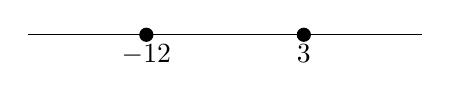
\begin{tikzpicture}
      \draw (0,0) -- (5,0);
      \node (a) [circle,draw,fill,scale=0.5] at (1.5,0) {};
      \node (b) [circle,draw,fill,scale=0.5] at (3.5,0) {};
      \node [below] at (a) {$-12$};
      \node [below] at (b) {$3$};
    \end{tikzpicture}

    $x=-12,3$
    
    \bigskip

  \item $x^2+9x-36<0$
    
    \bigskip

    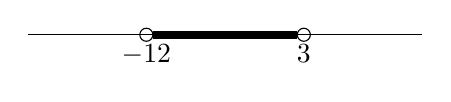
\begin{tikzpicture}
      \draw (0,0) -- (5,0);
      \node (a) [circle,draw,scale=0.5] at (1.5,0) {};
      \node (b) [circle,draw,scale=0.5] at (3.5,0) {};
      \node [below] at (a) {$-12$};
      \node [below] at (b) {$3$};
      \draw [line width=1mm] (a) to (b);
    \end{tikzpicture}

    $x\in(-12,3)$
    
    \bigskip

  \item $x^2+9x-36\ge0$

    \bigskip

    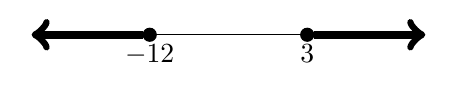
\begin{tikzpicture}
      \draw (0,0) -- (5,0);
      \node (a) [circle,draw,fill,scale=0.5] at (1.5,0) {};
      \node (b) [circle,draw,fill,scale=0.5] at (3.5,0) {};
      \node [below] at (a) {$-12$};
      \node [below] at (b) {$3$};
      \draw [->, line width=1mm] (a) to (0,0);
      \draw [->, line width=1mm] (b) to (5,0);
    \end{tikzpicture}

    $x\in(-\infty,-12]\cup[3,\infty)$

    \bigskip

  \end{enumerate}
  
\item Solve each of the following for $x$. Express your answers both
  graphically and in interval notation:
  \begin{enumerate}
  \item $\frac{x+3}{x-1}=0$

    \bigskip

    \begin{tikzpicture}
      \draw (0,0) -- (5,0);
      \node (a) [circle,draw,fill,scale=0.5] at (1.5,0) {};
      \node [below] at (a) {$-3$};
    \end{tikzpicture}

    $x=-3$

    \bigskip

  \item $\frac{x+3}{x-1}>0$
    
    \bigskip

    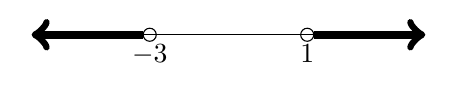
\begin{tikzpicture}
      \draw (0,0) -- (5,0);
      \node (a) [circle,draw,scale=0.5] at (1.5,0) {};
      \node (b) [circle,draw,scale=0.5] at (3.5,0) {};
      \node [below] at (a) {$-3$};
      \node [below] at (b) {$1$};
      \draw [->, line width=1mm] (a) to (0,0);
      \draw [->, line width=1mm] (b) to (5,0);
    \end{tikzpicture}

    $x\in(-\infty,-3)\cup(1,\infty)$
    
    \bigskip

  \item $\frac{x+3}{x-1}\le0$
    
    \bigskip

    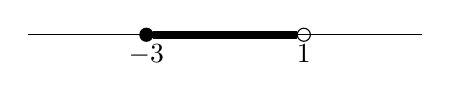
\begin{tikzpicture}
      \draw (0,0) -- (5,0);
      \node (a) [circle,draw,fill,scale=0.5] at (1.5,0) {};
      \node (b) [circle,draw,scale=0.5] at (3.5,0) {};
      \node [below] at (a) {$-3$};
      \node [below] at (b) {$1$};
      \draw [line width=1mm] (a) to (b);
    \end{tikzpicture}

    $x\in[-3,1)$
    
    \bigskip

  \end{enumerate}
  
\item Solve each of the following for $x$. Express your answers both
  graphically and in interval notation:
  \begin{enumerate}
  \item $3\abs{x-1}+1=7$

    $3\abs{x-1}=6$ \\
    $\abs{x-1}=2$ \\
    $x-1=\pm2$ \\
    $x=-1,3$
    
    \bigskip

    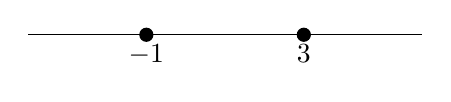
\begin{tikzpicture}
      \draw (0,0) -- (5,0);
      \node (a) [circle,draw,fill,scale=0.5] at (1.5,0) {};
      \node (b) [circle,draw,fill,scale=0.5] at (3.5,0) {};
      \node [below] at (a) {$-1$};
      \node [below] at (b) {$3$};
    \end{tikzpicture}

    $x=-1,3$
    
    \bigskip

  \item $3\abs{x-1}+1\le7$
    
    \bigskip

    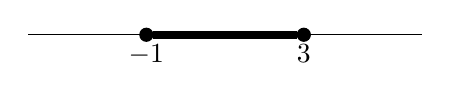
\begin{tikzpicture}
      \draw (0,0) -- (5,0);
      \node (a) [circle,draw,fill,scale=0.5] at (1.5,0) {};
      \node (b) [circle,draw,fill,scale=0.5] at (3.5,0) {};
      \node [below] at (a) {$-1$};
      \node [below] at (b) {$3$};
      \draw [line width=1mm] (a) to (b);
    \end{tikzpicture}

    $x\in[-1,3]$
    
    \bigskip

  \item $3\abs{x-1}+1\ge7$
    
    \bigskip

    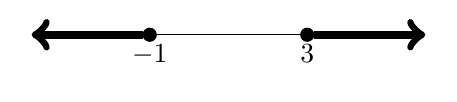
\begin{tikzpicture}
      \draw (0,0) -- (5,0);
      \node (a) [circle,draw,fill,scale=0.5] at (1.5,0) {};
      \node (b) [circle,draw,fill,scale=0.5] at (3.5,0) {};
      \node [below] at (a) {$-1$};
      \node [below] at (b) {$3$};
      \draw [->, line width=1mm] (a) to (0,0);
      \draw [->, line width=1mm] (b) to (5,0);
    \end{tikzpicture}

    $x\in(-\infty,-1]\cup[3,\infty)$
    
    \bigskip

  \end{enumerate}

\item Find the domain of the following expressions. Express your answers both
  graphically and in interval notation:
  \begin{enumerate}
  \item $\sqrt{\frac{x^2+2x-3}{x^2+5x+6}}$

    \bigskip

    This is an even root, so the radicand must be $\ge0$.
    
    \begin{eqnarray*}
      \frac{x^2+2x-3}{x^2+5x+6} &\ge& 0 \\
      \frac{(x+3)(x-1)}{(x+2)(x+3)} &\ge& 0 \\
      \frac{x-1}{x+2} &\ge& 0 \\
    \end{eqnarray*}
    Note: $x\ne-3$

    \bigskip

    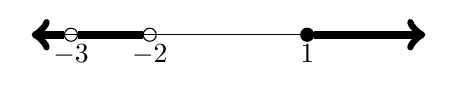
\begin{tikzpicture}
      \draw (0,0) -- (5,0);
      \node (a) [circle,draw,scale=0.5] at (1.5,0) {};
      \node (b) [circle,draw,fill,scale=0.5] at (3.5,0) {};
      \node (c) [circle,draw,scale=0.5] at (0.5,0) {};
      \node [below] at (a) {$-2$};
      \node [below] at (b) {$1$};
      \node [below] at (c) {$-3$};
      \draw [line width=1mm] (a) to (c);
      \draw [->, line width=1mm] (c) to (0,0);
      \draw [->, line width=1mm] (b) to (5,0);
    \end{tikzpicture}

    $x\in(-\infty,-3)\cup(-3,-2)\cup[1,\infty)$

    \bigskip

  \item $\sqrt[3]{\frac{x^2+2x-3}{x^2+5x+6}}$

    \bigskip

    This is an odd root, so we are only concerned a zero denominator.

    $(x+2)(x+3)\ne0$

    $x\ne-2,-3$

    \bigskip
    
    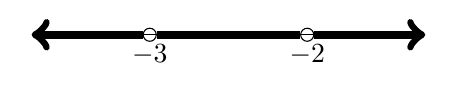
\begin{tikzpicture}
      \draw (0,0) -- (5,0);
      \node (a) [circle,draw,scale=0.5] at (1.5,0) {};
      \node (b) [circle,draw,scale=0.5] at (3.5,0) {};
      \node [below] at (a) {$-3$};
      \node [below] at (b) {$-2$};
      \draw [<-,line width=1mm] (0,0) to (a);
      \draw [line width=1mm] (a) to (b);
      \draw [->,line width=1mm] (b) to (5,0);
    \end{tikzpicture}

    \bigskip

    $x\in(-\infty,-3)\cup(-3,-2)\cup(-2,\infty)$

    \bigskip
      
  \end{enumerate}

\item Muri is a shopkeeper that specializes in pickled vegetables. She has
  determined over the years that the best brine (salt solution) for pickling
  vegetables is 2 kg of salt per liter of water (2 kg/L).  One day, she has her
  not-so-bright nephew helping her and he uses too much salt, resulting in
  a 5 kg/L solution.  If her nephew made up 10 liters of the too-salty solution,
  how much pure water must he add to it to get the ideal 2 kg/L solution? For
  full credit, show the mixture equation and the appropriate values for each
  concentration and volume value in the equation.

  \bigskip

  $c_1v_1+c_2v_2=c_3(v_1+v_2)$

  \begin{tabular}{cc}
    $c_1$ & $\SI{5}{kg/L}$ \\
    $v_1$ & $\SI{10}{L}$ \\
    $c_2$ & $\SI{0}{kg/L}$ \\
    $v_2$ & $x$ \\
    $c_3$ & $\SI{2}{kg/L}$ \\
    $v_1+v_2$ & $10+x$
  \end{tabular}

  $5(10)+0x=2(10+x)$ \\
  $50=2(10+x)$ \\
  $x+10=25$
  
  $x=15$

  Thus, $\SI{15}{L}$ of pure water must be added to the $\SI{10}{L}$ of
  $\SI{5}{kg/L}$ solution in order to dilute it to $\SI{2}{kg/L}$.
\end{enumerate}

\end{document}
